%%%%%%%%%%%%%%%%%%%%%%%%%%%%%%%%%%%%%%%%%
% Journal Article
% LaTeX Template
% Version 1.3 (9/9/13)
%
% This template has been downloaded from:
% http://www.LaTeXTemplates.com
%
% Original author:
% Frits Wenneker (http://www.howtotex.com)
%
% License:
% CC BY-NC-SA 3.0 (http://creativecommons.org/licenses/by-nc-sa/3.0/)
%
%%%%%%%%%%%%%%%%%%%%%%%%%%%%%%%%%%%%%%%%%

%----------------------------------------------------------------------------------------
%	PACKAGES AND OTHER DOCUMENT CONFIGURATIONS
%----------------------------------------------------------------------------------------

\documentclass[twoside]{article}

\usepackage{graphicx}
\usepackage{lipsum} % Package to generate dummy text throughout this template

\usepackage[sc]{mathpazo} % Use the Palatino font
\usepackage[T1]{fontenc} % Use 8-bit encoding that has 256 glyphs
\linespread{1.05} % Line spacing - Palatino needs more space between lines
\usepackage{microtype} % Slightly tweak font spacing for aesthetics

\usepackage[hmarginratio=1:1,top=32mm,columnsep=20pt]{geometry} % Document margins
\usepackage{multicol} % Used for the two-column layout of the document
\usepackage[hang, small,labelfont=bf,up,textfont=it,up]{caption} % Custom captions under/above floats in tables or figures
\usepackage{booktabs} % Horizontal rules in tables
\usepackage{float} % Required for tables and figures in the multi-column environment - they need to be placed in specific locations with the [H] (e.g. \begin{table}[H])
\usepackage{hyperref} % For hyperlinks in the PDF

\usepackage{lettrine} % The lettrine is the first enlarged letter at the beginning of the text
\usepackage{paralist} % Used for the compactitem environment which makes bullet points with less space between them
\usepackage{amsmath}
\usepackage{abstract} % Allows abstract customization
\renewcommand{\abstractnamefont}{\normalfont\bfseries} % Set the "Abstract" text to bold
\renewcommand{\abstracttextfont}{\normalfont\small\itshape} % Set the abstract itself to small italic text

\usepackage{titlesec} % Allows customization of titles
\renewcommand\thesection{\Roman{section}} % Roman numerals for the sections
\renewcommand\thesubsection{\Roman{subsection}} % Roman numerals for subsections
\titleformat{\section}[block]{\large\scshape\centering}{\thesection.}{1em}{} % Change the look of the section titles
\titleformat{\subsection}[block]{\large}{\thesubsection.}{1em}{} % Change the look of the section titles

\usepackage{fancyhdr} % Headers and footers
\pagestyle{fancy} % All pages have headers and footers
\fancyhead{} % Blank out the default header
\fancyfoot{} % Blank out the default footer
\fancyhead[C]{PHSX567 Final Project Progress Report $\bullet$ \today } % Custom header text
\fancyfoot[RO,LE]{\thepage} % Custom footer text
\usepackage{subcaption}

%----------------------------------------------------------------------------------------
%	TITLE SECTION
%----------------------------------------------------------------------------------------

\title{\vspace{-15mm}\fontsize{24pt}{10pt}\selectfont\textbf{Progress Report for MOSES Data Inversion with CNNs}} % Article title

\author{
\large
\textsc{Roy Smart}\\[2mm] % Your name
\normalsize Montana State University \\ % Your institution
\normalsize \href{mailto:roytsmart@gmail.com}{roytsmart@gmail.com} % Your email address
\vspace{-5mm}
}
\date{}

%----------------------------------------------------------------------------------------

\begin{document}

\maketitle % Insert title

\thispagestyle{fancy} % All pages have headers and footers



%----------------------------------------------------------------------------------------
%	ARTICLE CONTENTS
%----------------------------------------------------------------------------------------

\section{Introduction}

Simplified MOSES data inversion was attempted using a convolutional neural networks.  Data was prepared randomly and then fed through the MOSES forward model. Results from the forward model were used as input to a convolutional neural network and then compared to the input of the MOSES forward model to train the network. This test was very successful, achieving very high accuracy. While this is a very simple example of MOSES data inversion, it is an important step to learning how to use convolutional neural networks.

\section{Data Preparation}

 The MOSES instrument observes the sun in spatial directions $x$ and $y$. This measurement is the projection of a spectral cube in $x$, $y$, and $\lambda$. In the MOSES coordinate system $x$ is the dispersion direction. Therefore, (if we neglect the point-spread function,) we may ignore the $y$ component of the images without loss of generality. \par For this test we randomly construct a slice of the spectral cube in $x$ and $\lambda$, with dimensions 4 by 4. We will call this image the "truth" image, and the output of the neural network should strive to create this image. 
 
 \begin{figure}[H]
   
   \centering
     
\includegraphics[width=0.5\textwidth]{images/mIn}
     \caption{An example of a 4 pixel by 4 pixel truth image.}
     \label{mIn}
 \end{figure}
 
 From the truth image, we simulate the measurements captured by the instrument using the so-called MOSES forward model (fomod). Fomod works by summing along each spectral direction for the $m=0$, $1$, and $-1$ spectral orders. Since the $y$ dimension has been ignored, we are left with a graph, described in Figure \ref{m1-1}
 
 \begin{figure}
     \centering
     \begin{subfigure}[b]{0.3\textwidth}
         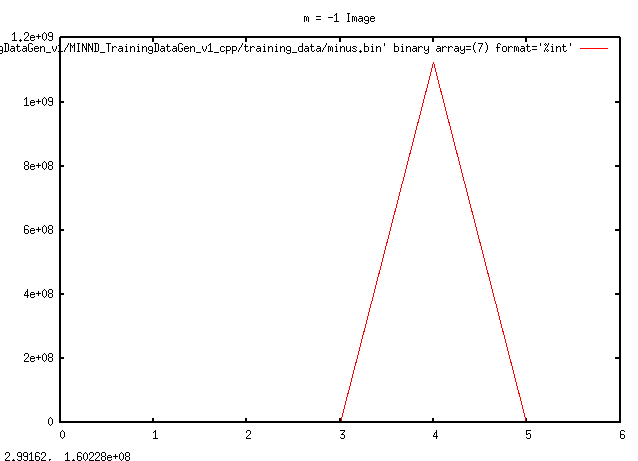
\includegraphics[width=\textwidth]{images/m-1}
         \caption{$m = -1$ order }
     \end{subfigure}
      \begin{subfigure}[b]{0.3\textwidth}
          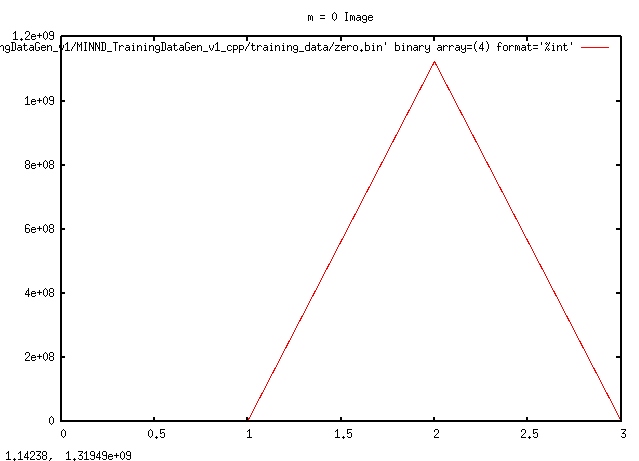
\includegraphics[width=\textwidth]{images/m0}
          \caption{$m = 0$ order }
      \end{subfigure}
        \begin{subfigure}[b]{0.3\textwidth}
            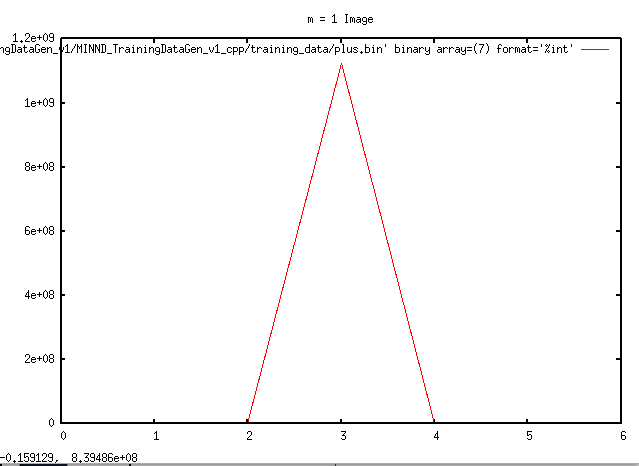
\includegraphics[width=\textwidth]{images/m1}
            \caption{$m = 1$ order }
        \end{subfigure}
 
     \caption{Simulated results of the MOSES instrument for the simple case described in Figure \ref{mIn}.}
     \label{m1-1}
 \end{figure}
 
 Unfortunately, convolutional neural networks do not work as well on graphs, they are designed to work with images. We can transform the graphs from the three orders back into an image by backprojecting along each spectral direction. The result is essentially an image that contains the maximum possible pixel value at every location in the spectral slice. For our purposes we will store the projections from each order on separate color channels (RGB). We will call this image the "input" image, and it will be the image that is fed into the neural network. An example of this image is given in Figure \ref{mOut}. This process gives the neural network important information about the operation of the MOSES forward model and may help the network train faster. 
 
  \begin{figure}[H]
    
    \centering
      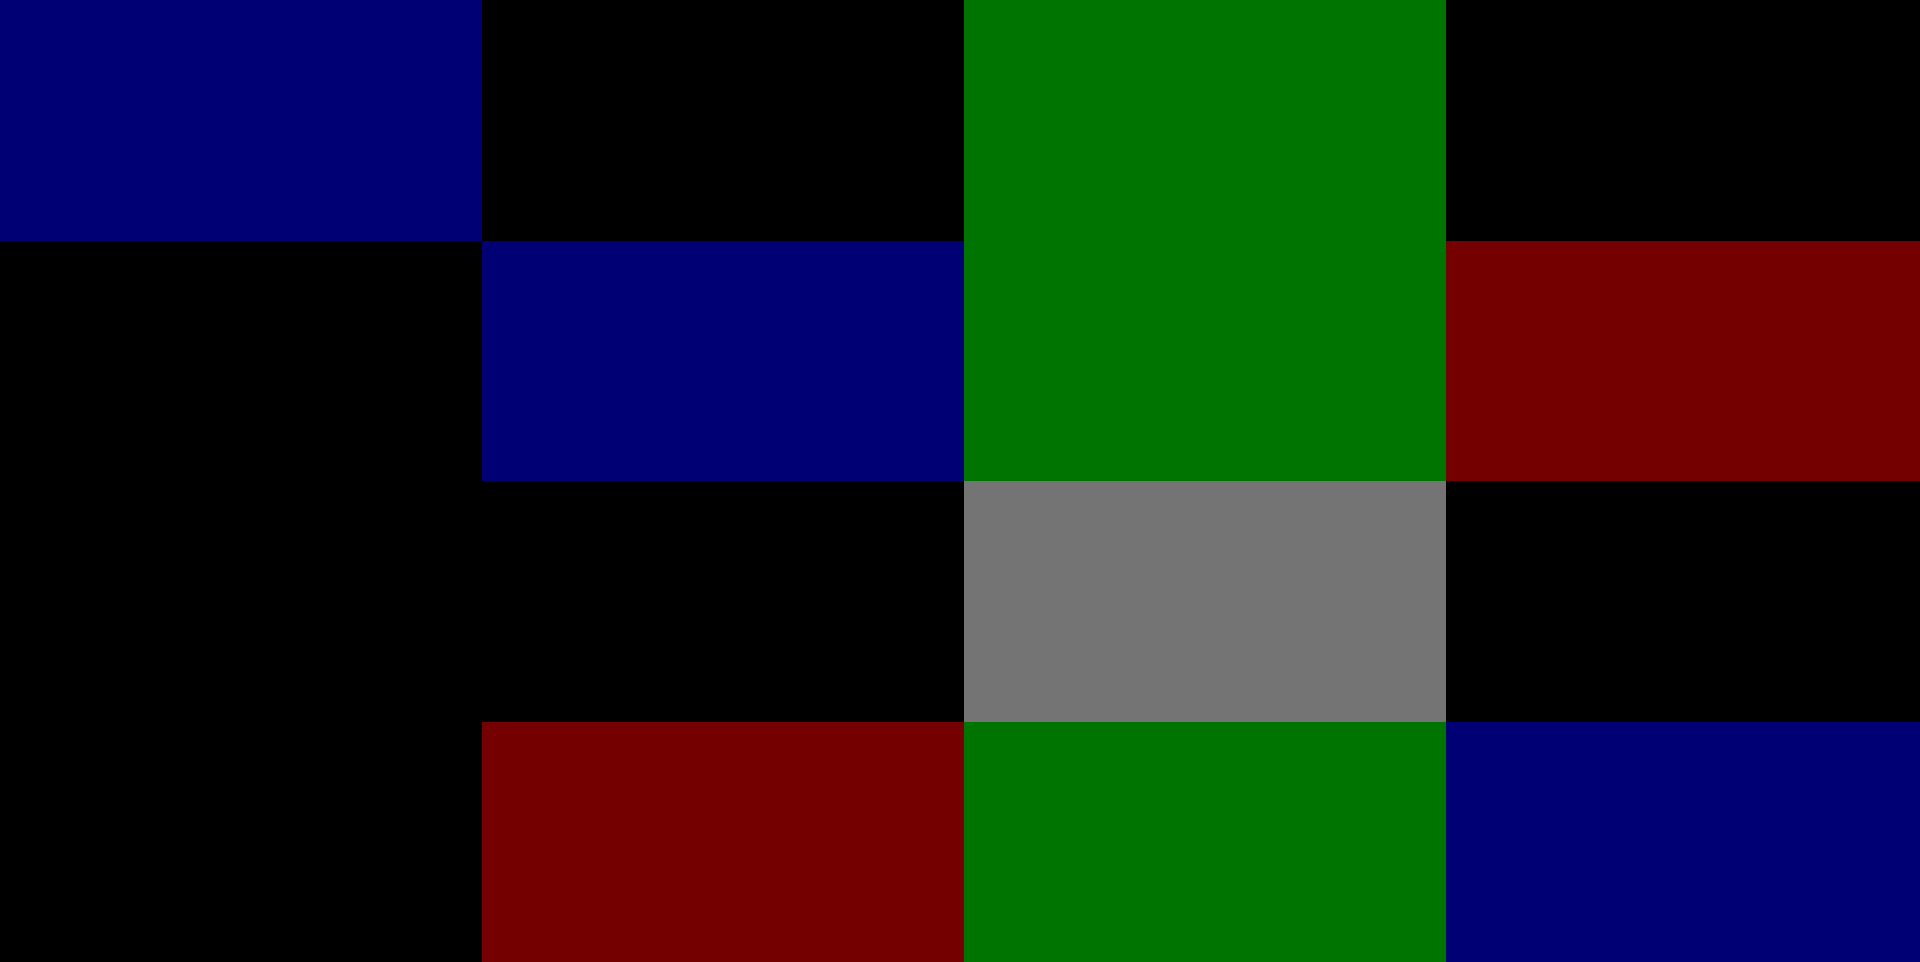
\includegraphics[width=0.5\textwidth]{images/mOut}
      \caption{An example of a 4 pixel by 4 pixel input image.}
      \label{mOut}
  \end{figure}
 
 We created 10,000 4 by 4 pixel, 8 bits per pixel truth-input image pairs and used them to train the network.
 
\section{Neural Network Architecture}

The neural network architecture was slightly arbitrary, in that we haven't had too much time to explore the hyperparameter space. The architecture we developed consisted of one convolutional layer, one max pooling layer, followed by three fully connected layers, with ReLU layers in between. This is outlined in Figure \ref{net}.

  \begin{figure}[H]
    
    \centering
      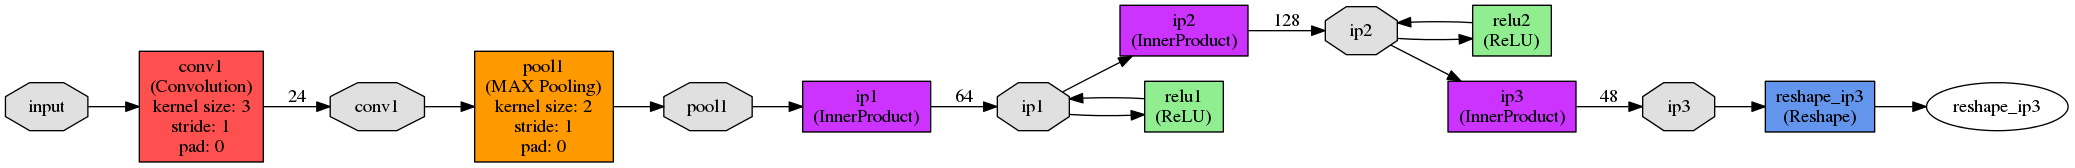
\includegraphics[width=\textwidth]{images/net}
      \caption{Flow chart of the layout of the neural network used for this test.}
      \label{net}
  \end{figure}
  
  The performance of each layer is not yet understood very well, and will become more clear as the image size and complexity increases. However, we will explain the intended effect of each layer here. The convolutional layer should consist of a series of orthogonal filters described in Figure \ref{ortho}.
  
    \begin{figure}[H]
      
      \centering
        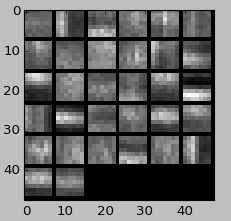
\includegraphics[width=0.5\textwidth]{images/ortho}
        \caption{Example of orthogonal filters in convolutional layer. NOTE: This is not from out network.}
        \label{ortho}
    \end{figure}
    
The max pooling layer helps determine which convolutional filter is most prevalent. In larger/more complex images, there will be more convolutional/max pooling layers to handle the information increase. \par After the max pooling layers, the information is fed into a more classical neural network, with each neuron fully connected to one another. (In Caffe terms, thi s a fully-connected layer is called an inner product layer.) This layer takes the information from the convolutional filter output and reconstructs the truth image.

\section{Results}

\subsection{4 x 4 Pixels, 1 active pixel}
The network was trained for 10,000 iterations. Each truth image was 4 by 4 pixels and had one active pixel between the values of 0 and 255 randomly placed on the image. The loss computed by Caffe after 10,000 iterations was 5.38543e-05. Since $4 \times 4 \times 255 = 4080$, it is likely that the neural network simply memorized the training dataset.

\begin{table}[H]
\begin{tabular}{| r | c | c | c | c |}
\hline
Iteration & Input & Output & Truth & Difference \\ \hline
1 & 
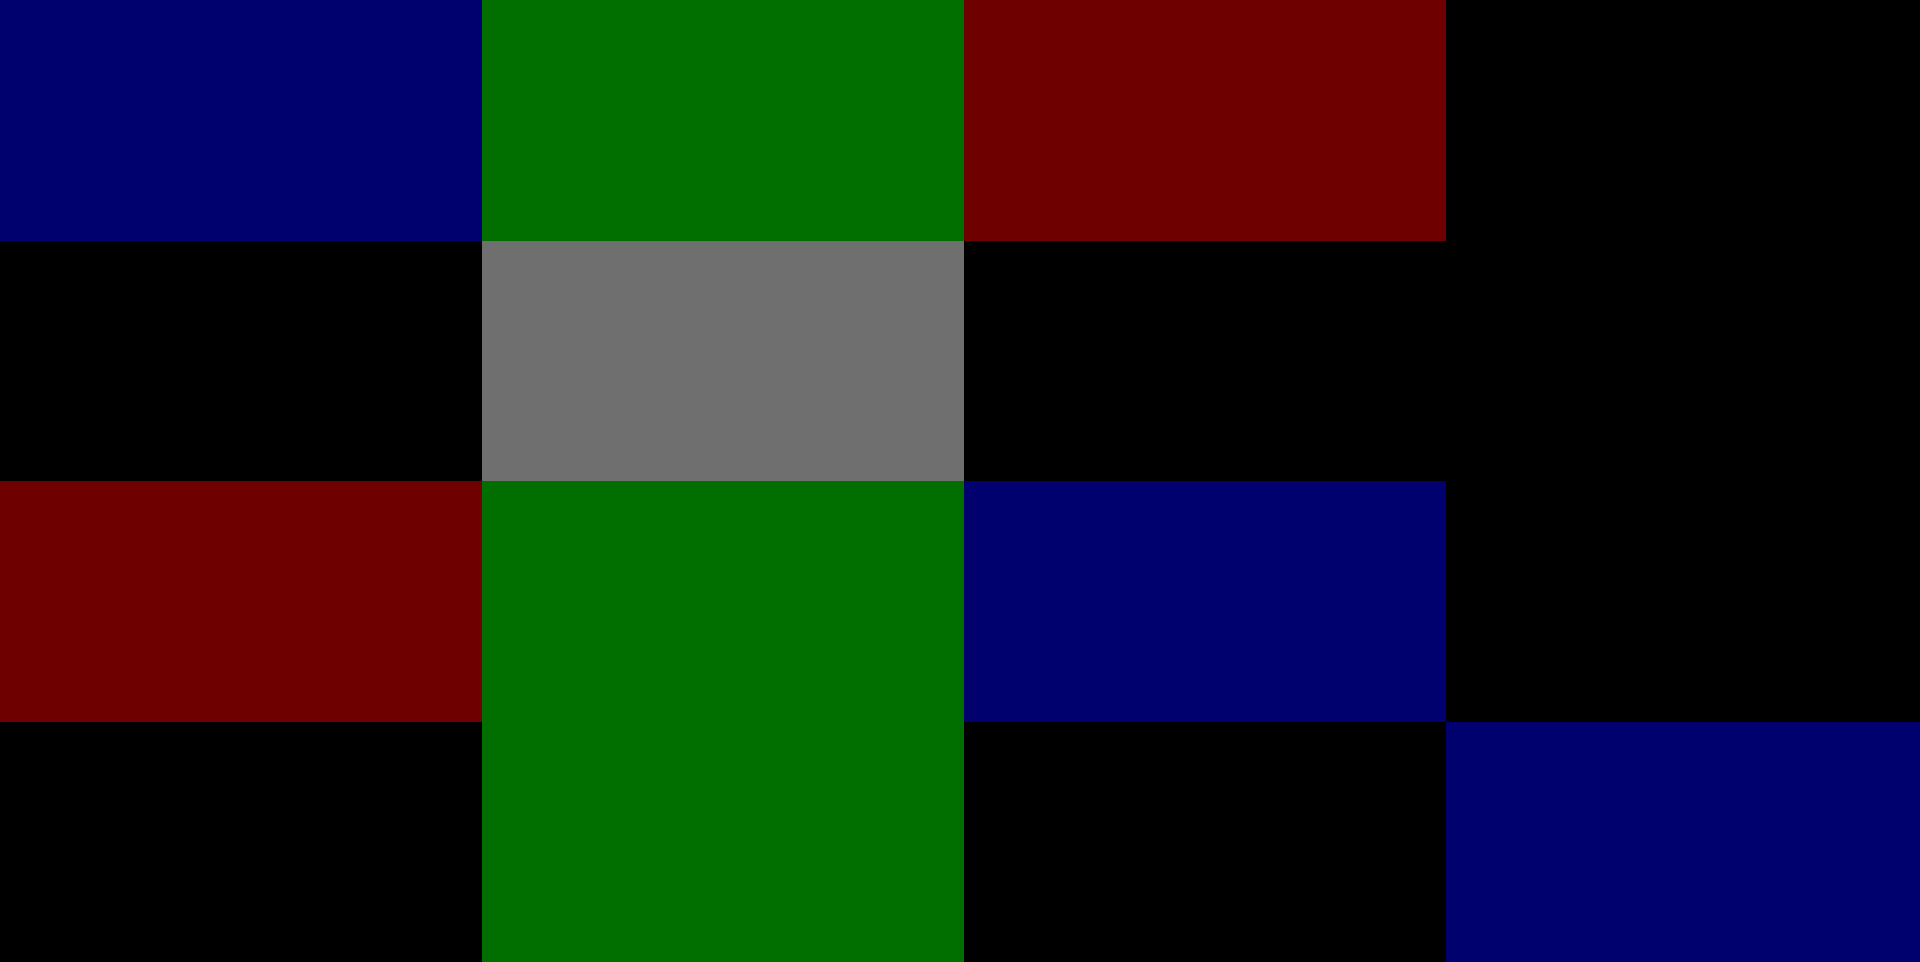
\includegraphics[width=0.2\textwidth]{images/4x4/1/in} &

\includegraphics[width=0.2\textwidth]{images/4x4/1/out} &

\includegraphics[width=0.2\textwidth]{images/4x4/1/truth} &

\includegraphics[width=0.2\textwidth]{images/4x4/1/dif} \\ \hline
\end{tabular}
\caption{Characteristic output for the 4x4 case. MINND performs perfectly each time.}
\end{table}

\subsection{8 x 8 Pixels, Up to 5 active pixels}

For this size of image, we used the network configuration described in Figure \ref{net8x8}.

    \begin{figure}[H]
      
      \centering
        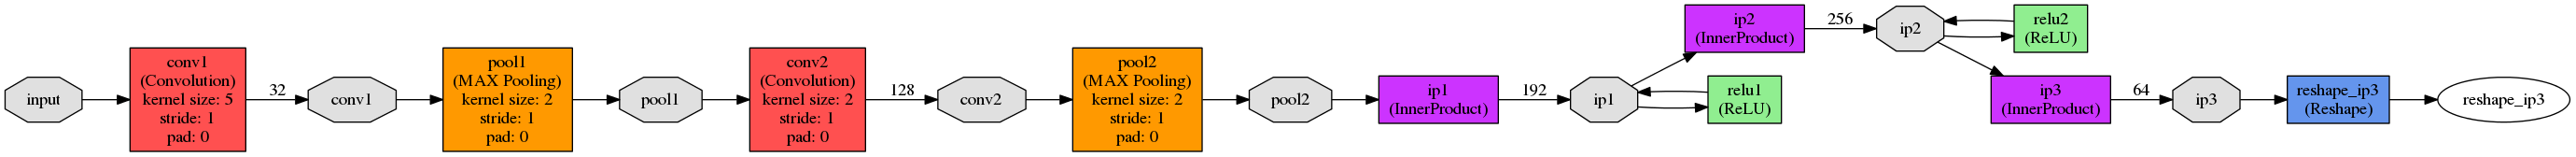
\includegraphics[width=\textwidth]{images/8x8/minnd_dia}
        \caption{Neural Network configuration for 8x8 pixel input/output image}
        \label{net8x8}
    \end{figure}
  The network was trained for 1 million iterations. Each truth image was 8 by 8 pixels and had between 1 and 5 active pixels between the values of 0 and 255 randomly placed on the image. The loss computed by Caffe after 1,000,000 iterations was 0.127717. \par This is much worse than the 4x4 case reported above. This is to be expected as there are many possible solutions to any non-trivial input image. However, the neural network doesn't perform perfectly, as the neural network output isn't necessarily a solution to an input cube.

\begin{table}[H]
\begin{tabular}{| r | c | c | c | c |}
\hline
Iteration & Input & Output & Truth & Difference \\ \hline
1 & 
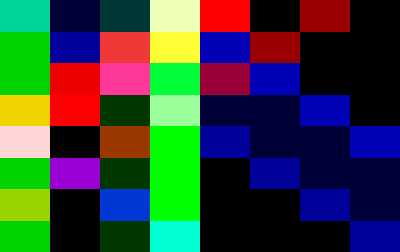
\includegraphics[width=0.2\textwidth]{images/8x8/1/in} &

\includegraphics[width=0.2\textwidth]{images/8x8/1/out} &
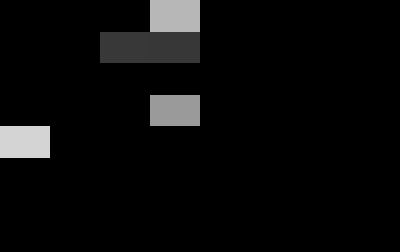
\includegraphics[width=0.2\textwidth]{images/8x8/1/truth} &

\includegraphics[width=0.2\textwidth]{images/8x8/1/dif} \\ \hline
2 & 
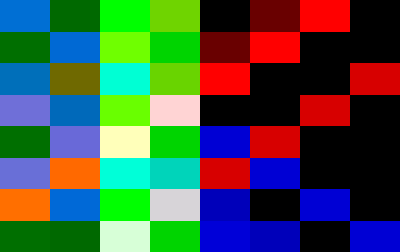
\includegraphics[width=0.2\textwidth]{images/8x8/2/in} &

\includegraphics[width=0.2\textwidth]{images/8x8/2/out} &
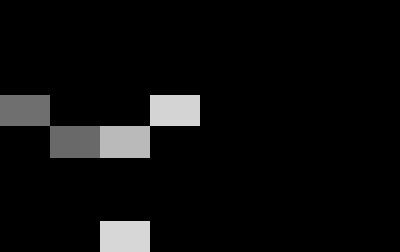
\includegraphics[width=0.2\textwidth]{images/8x8/2/truth} &

\includegraphics[width=0.2\textwidth]{images/8x8/2/dif} \\ \hline
3 & 
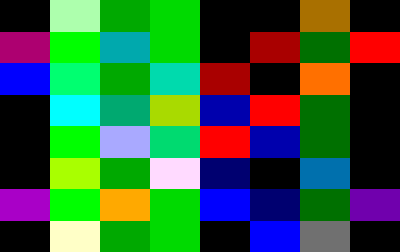
\includegraphics[width=0.2\textwidth]{images/8x8/3/in} &

\includegraphics[width=0.2\textwidth]{images/8x8/3/out} &
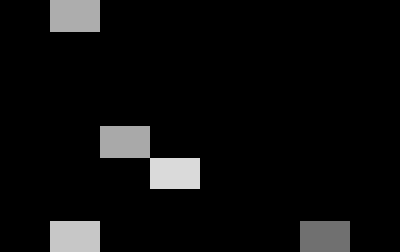
\includegraphics[width=0.2\textwidth]{images/8x8/3/truth} &

\includegraphics[width=0.2\textwidth]{images/8x8/3/dif} \\ \hline
4 & 
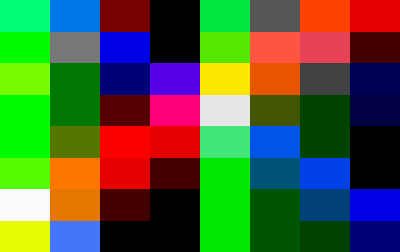
\includegraphics[width=0.2\textwidth]{images/8x8/4/in} &

\includegraphics[width=0.2\textwidth]{images/8x8/4/out} &
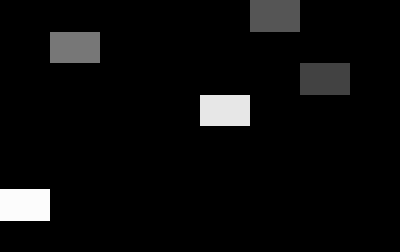
\includegraphics[width=0.2\textwidth]{images/8x8/4/truth} &

\includegraphics[width=0.2\textwidth]{images/8x8/4/dif} \\ \hline
\end{tabular}
\caption{Output of the MINND neural network for four randomly selected input images. Notice how not all output images are solutions to the inversion problem.}
\end{table}
\section{Conclusion}

We have proved that a neural network can give a reasonable answer to the MOSES inversion problem for simple datasets.  The network performed really well in the 1 active pixel getting the right answer every time. However the performance was disappointing in the 5 active pixel case, not only getting the answer wrong, but the solution presented by the network was not a potential solution to the inversion problem. \par The performance of the network could potentially be improved in many ways. Selection of hyperparameters such as convolutional kernel size, learning rate, and number of hidden neurons may all help to increase the accuracy of the network. Also, the size of the training dataset was fairly small, consisting of only 1 million images in the 8x8 case. It is possible that larger training datasets will allow for better convergence. \par Furthermore while the data presented to this neural network was completely random, the next dataset (the IRIS dataset) will have a structure with solar characteristics. This will provide details for the neural network to recognize, trimming potential solutions to the inversion problem.

	\bibliographystyle{unsrt}
	\bibliography{sources}
\end{document}
